\chapter{First Chapter}
This test sentence is supposed to span more than one line.
Or maybe, we need another sentence for this.
And why, you ask, do we need several lines at all?
Well, to test the line spacing, of course!
Let's have a citation \cite{kalman1960new} and another one here \cite{nowak2003efficient}.

We can have enumerations:
\begin{enumerate}
    \item First important item.
    \item Second important item.
\end{enumerate}
and lists:
\begin{itemize}
    \item Item one.
    \item Item two.
\end{itemize}
or how about a description:
\begin{description}
    \item[big] is the opposite of small.
    \item[small] is the opposite of big.
\end{description}

\minisec{A mini section}
Gives you a small heading that isn't separated too much from the previous text.
This section is not part of the index.
Please have a look at table ~\ref{table:example} on page ~\pageref{table:example}.
Alternatively, we can use `vref` to expand a reference automatically, if necessary:
see table ~\vref{table:example}.
See the `vref` documentation for more handy reference options.

Talking about references, just use `vref` all the time, also for equations.
The package `amsmath` defines `eqref` which automatically returns parenthes around the equation number, but in this document we have defined `vref` to do the same.
See equation ~\vref{eq:trig}.

\begin{table}
    \centering
    \begin{tabular}{llll}
        This & is & an & example. \\\hline
        Just & useless & content & here.
    \end{tabular}
    \caption{An example table.}
    \label{table:example}
\end{table}

\section{Equations}
The `amsmath` package provides several environments for equations.
For each environment, there is also a starred version that does not use automatic numbering.
For a single equation that spans a single line use the `equation` environment:
\begin{equation}
    \label{eq:circle}
    x^2 + y^2 = r^2
\end{equation}

`gather` is used for several equations that should not be aligned:
\begin{gather}
    x^2 + y^2 = r^2 \\
    r = 1
\end{gather}

`align` is used for several equations that should be aligned:
\begin{align}
    r^2 &= x^2 + y^2 \\
    r &= 1
\end{align}

If one of your equations gets too long, check out the `multiline` (no alignment) and `split` environments (with alignment).
These environments don't enumerate each line of the equation (which could be supressed using `\textbackslash notag`).

\section{Figures}
In general use floating figures with the `figure` environment.
See \href{https://tex.stackexchange.com/questions/39017/how-to-influence-the-position-of-float-environments-like-figure-and-table-in-lat}{this} article for an explanation of how Latex places floating figures.
If you want to display two figures or tables next to each other, you either need to use minipages (see the `subcaption` docs) or the `subfigure` and `subtable` environments.
Of course, we can now again reference both subfigures ~\vref{fig:subfig_a} and ~\vref{fig:subfig_b}, as well as the whole figure ~\vref{fig:subfig}.
\begin{figure}
    % If you don't use the [b] option, the subfigures won't be placed on the
    % bottom of the figure minipage.
    \begin{subfigure}[b]{0.5\textwidth}
        \centering
				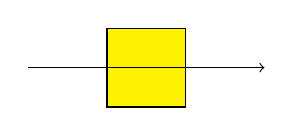
\begin{tikzpicture} % Simple figures can also be created using the tikz package.
					\draw[fill=yellow] (0,0) -- (0,1) -- (1,1) -- (1,0) -- cycle;
					\draw [->] (-1,0.5) -- (2,0.5);
				\end{tikzpicture}
        \caption{The first subfigure}\label{fig:subfig_a}
    \end{subfigure}
    \begin{subfigure}[b]{0.5\textwidth}
        \centering
        % \linewidth now is the width of this subfigure environment
        
\includegraphics[width=\linewidth]{images/logo_unis_de.pdf}
        \caption{The second subfigure}\label{fig:subfig_b}
    \end{subfigure}
\caption{A figure with two subfigures}
\label{fig:subfig}
\end{figure}

When defining the width of figures, the following lengths may be useful:
\begin{description}
    \item[\textbackslash linewidth] The width of a line in the \emph{current} environment.
    \item[\textbackslash columnwidth] The width of a column (in a multi-column document).
    \item[\textbackslash textwidth] The width of the text on the page.
    \item[\textbackslash paperwidth] Self-explanatory.
\end{description}

If you use inkscape for your images you may want to use the `svg` file format.
Have a look at the `svg` package to do so - it has some nice features.
One of them is to automatically save the rendered vector image in the same size as, e.g., a pdf file.
This is handy, because it allows you to give a copy of a figure of the exact same size as in your document to someone else.

\section{Source Code Listings}
The `listings` package provides syntax highlighting for source code.
It allows you to include an external file, you can use inline code
(\lstinline[language=matlab]!sqrt(x.^2)!)
or use its environment `lstlisting`:

\begin{lstlisting}[language=matlab, title={A simple MATLAB program.}]
for i = 1:10
    fprintf('Look, a number: %i\n', i);
end
\end{lstlisting}

It is probably better to use a floating environment for bigger listings, like the Python code example ~\vref{code:python_ex}.
Also, in the Matlab example we didn't set a caption, but a title.
This means that it is not listed in the list of listings and that it does not receive a code listing number.
\begin{lstlisting}[float, language=python, caption={A simple Python program.},
                   label=code:python_ex]
for i in range(10):
    print('Look, a number: %i' % i)
\end{lstlisting}
